
\chapter{Plugin}

    I plugin aggiungono funzionalita' aggiuntive ad Unreal Engine.

    Esistono plugin:
    \begin{itemize}
        \item gia' inclusi in Unreal Engine: non bisogna installarli
        \item da installare mediante interfaccia di Unreal Engine andando su:

            \begin{lstlisting}
                Edit > Plugins
            \end{lstlisting}

            Verra' aperta la schermata nella figura \ref{fig:unreal_editor_plugins}.

        \item da installare scaricandoli, ad esempio da GitHub, e posizionandoli nella cartella "Plugins" del progetto
    \end{itemize}


    % GEOMETRY SCRIPT
    \section{Geometry Script}

        Permette di creare delle mesh dinamiche semplici.


    % DATASMITH
    \section{Datasmith}

        I plugin Datasmith permettono di importare in Unreal Engine formati che non sono supportati di default.

        \subsection{Datasmith CAD importer}

            Permette di importare file AutoCAD.


    % MQTT UTILITIES
    \section{MQTT Utilities}

        \href{https://github.com/NinevaStudios/mqtt-utilities-unreal}{"MQTT Utilities"} e' un plugin scaricabile da GitHub che aggiunge ad Unreal Engine
        la possibilita' di gestire il protocollo MQTT (inviare e ricevere messaggi dal broker).

        \begin{warningbox}
            L'attuale ultima versione, ovvero la v1.1.0, ha un bug che fa crashare l'engine.

            Se non sono presenti nuove release e' consigliato scaricare il plugin direttamente dal branch master:
            il codice del branch master ha il bug fix che risolve il problema.
        \end{warningbox}

        Per installare il plugin occorre:
        \begin{enumerate}
            \item Scaricarlo
            \item Creare, se non esiste, una cartella "Plugins" all'interno della cartella del progetto Unreal Engine
            \item Creare una cartella per il plugin chiamata "mqtt-utilities-unreal" e spostare i file della root del plugin al suo interno.

                \begin{notebox}
                    Ad esempio se si sta lavorando su un progetto chiamato "DigitalShadowLED" navigare nella sua cartella (quella che contiene il file ".uproject").

                    Il file README dovra' essere posizionato all'interno della cartella:

                    \begin{lstlisting}
                        DigitalShadowLED\Plugins\mqtt-utilities-unreal
                    \end{lstlisting}

                    Dove "DigitalShadowLED" e' la cartella contenente il file ".uproject".
                \end{notebox}

            \item Aprire Unreal Engine
            \item Aprire la lista dei plugin (figura \ref{fig:unreal_editor_plugins}) e abilitare il plugin da:

                \begin{lstlisting}
                    Edit > Plugins > Code Plugins
                \end{lstlisting}

            \item Aprire il file che termina con "Build.cs" (presente nella sottocartella contenuta nella cartella "Source") e modificare la seguente riga in modo da contenere "MqttUtilities":

                \begin{minted}[autogobble]{csharp}
                    PublicDependencyModuleNames.AddRange(new string[] { "Core", ... , "MqttUtilities" });
                \end{minted}
        \end{enumerate}


    % FIGURE

    \begin{figure}[h]
        \caption{Unreal Engine: Plugin}
        \centering
        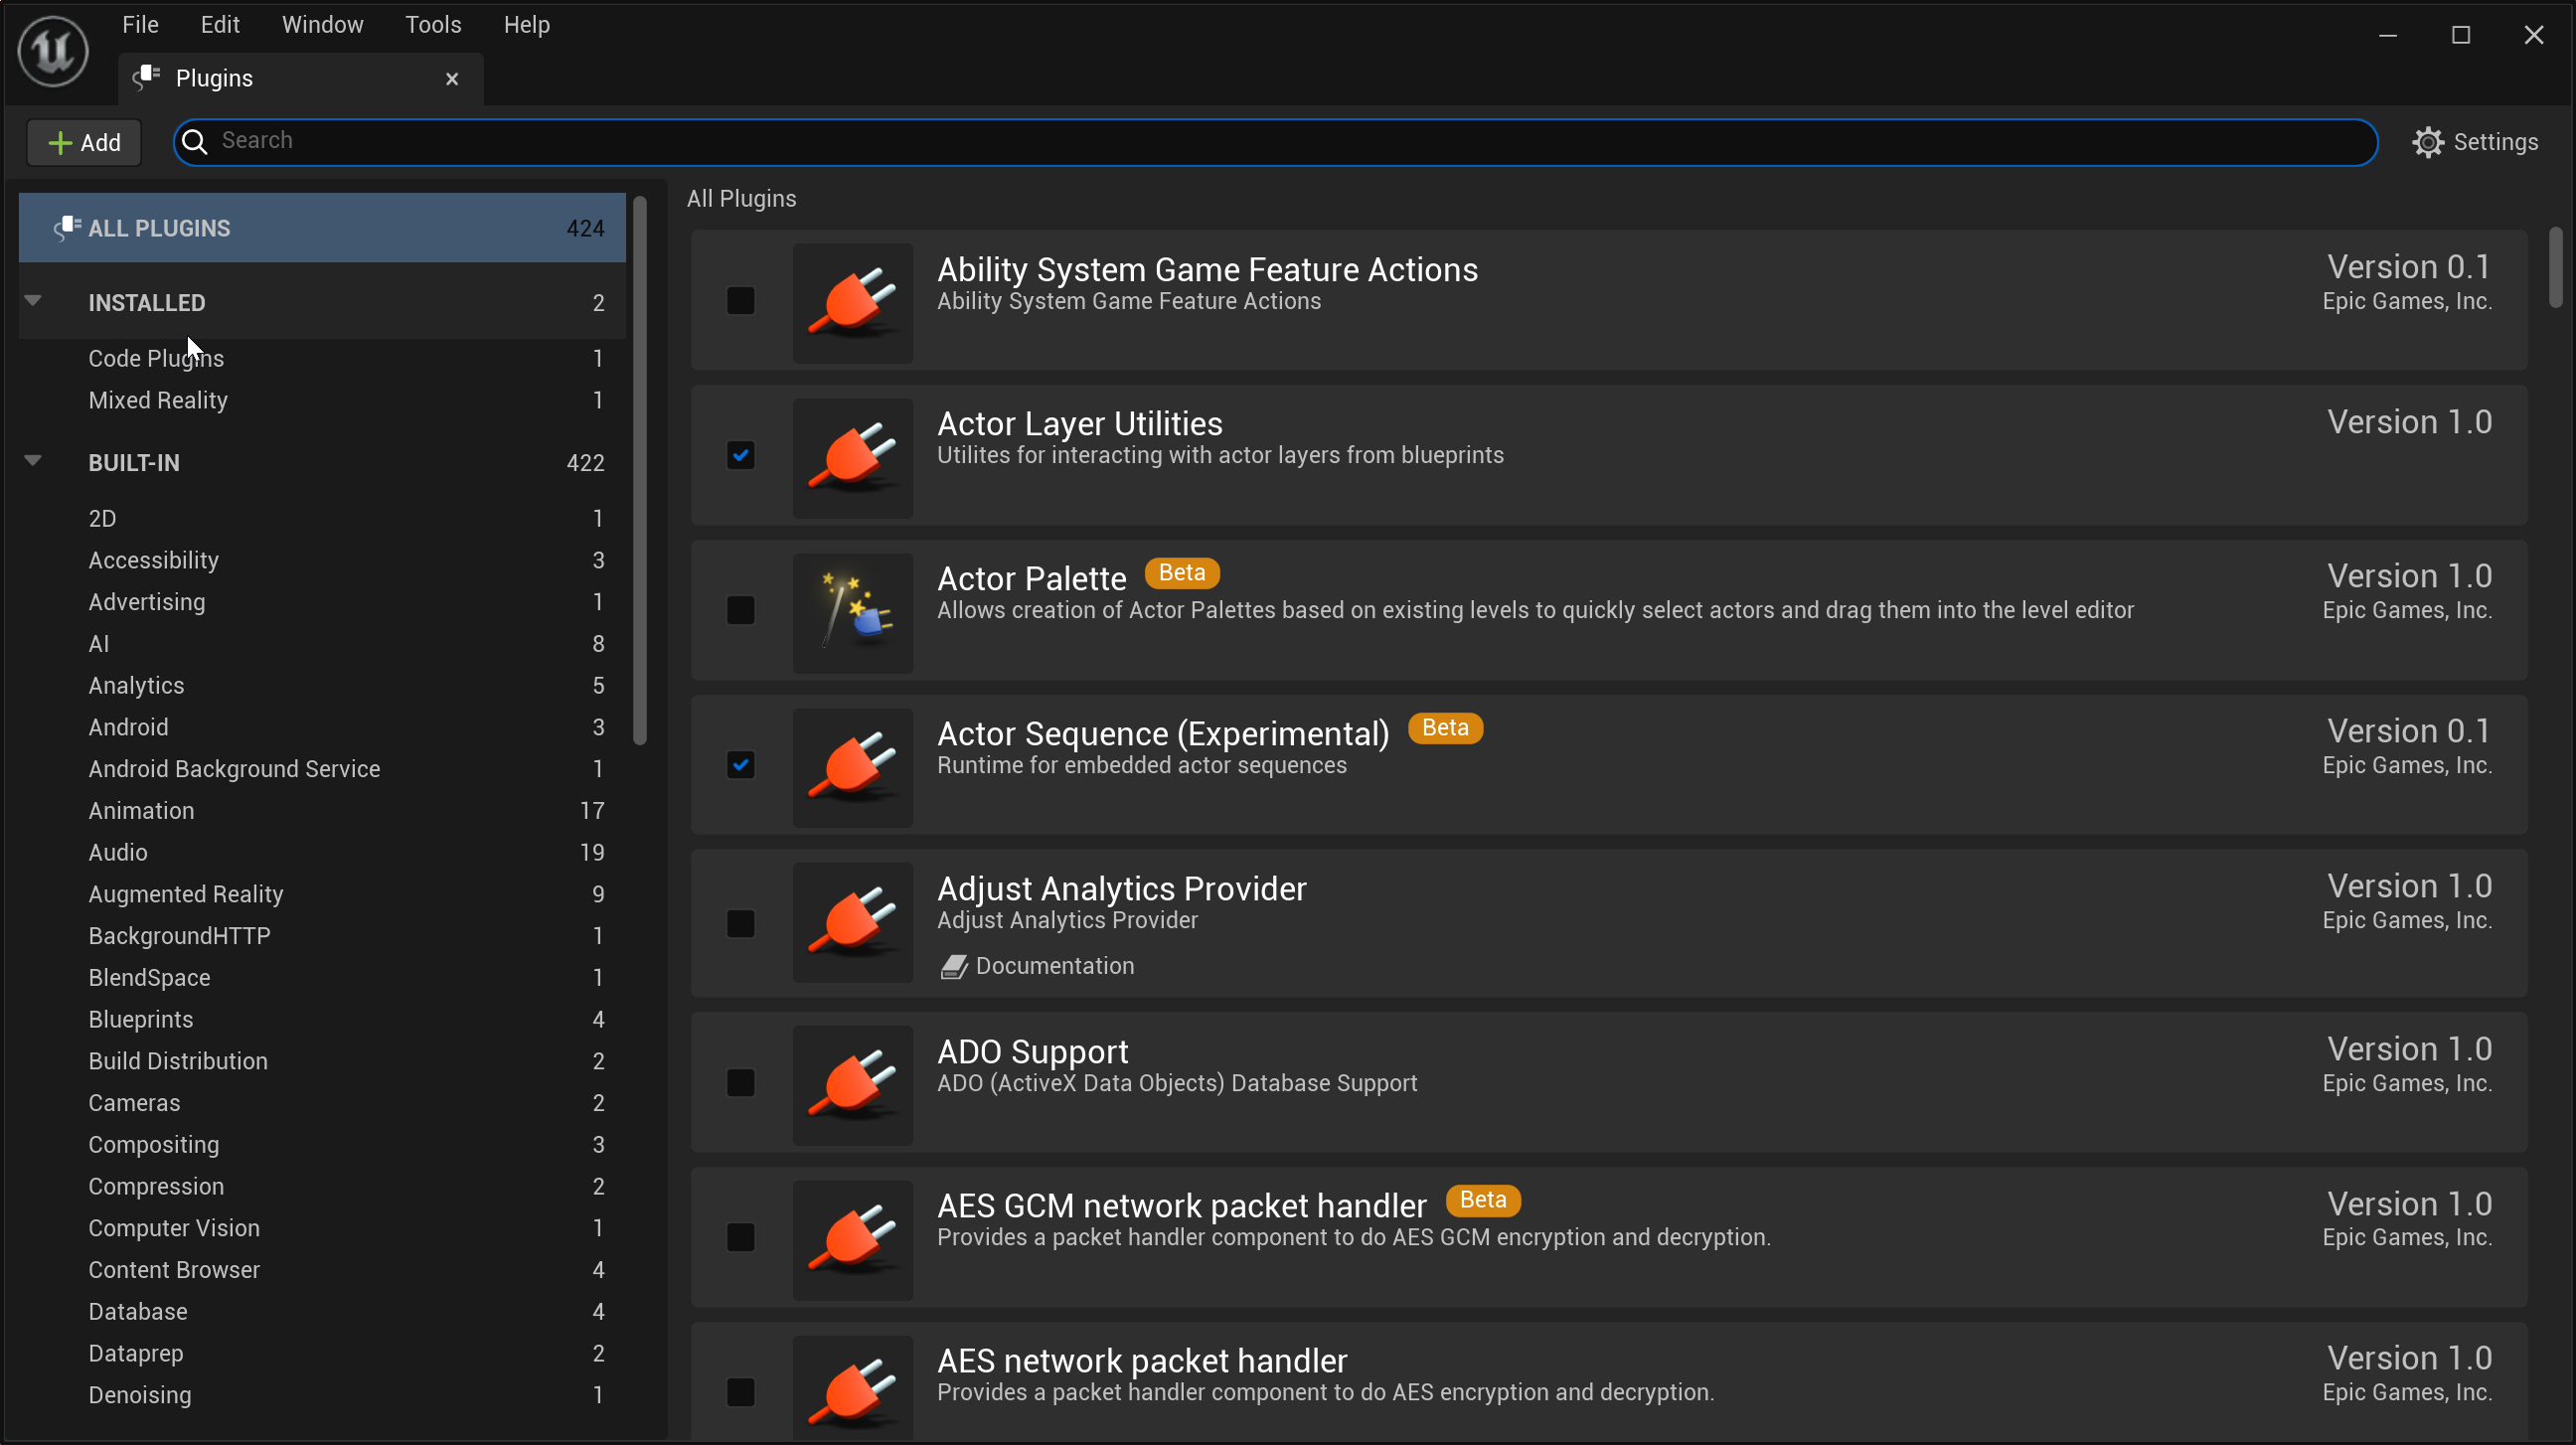
\includegraphics[width=\textwidth]{ue_plugins}
        \label{fig:unreal_editor_plugins}
    \end{figure}
